\documentclass{standalone}
\usepackage{tikz-network}

\begin{document}
    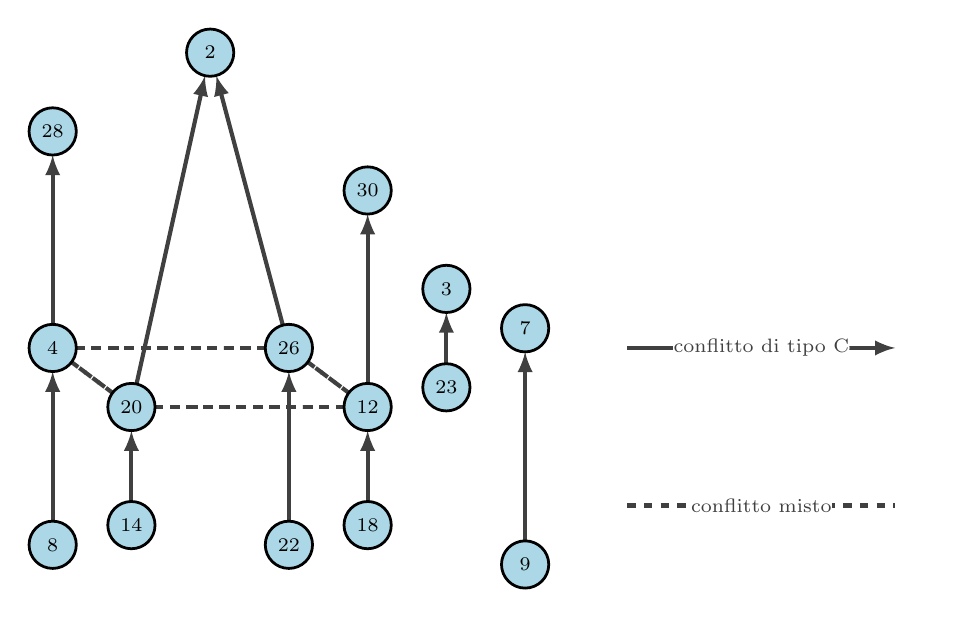
\begin{tikzpicture}
        \Vertex[x=2, y=27/4, label=$2$]{2}
        \Vertex[x=5, y=15/4, label=$3$]{3}
        \Vertex[x=0, y=12/4, label=$4$]{4}
        \Vertex[x=6, y=13/4, label=$7$]{7}
        \Vertex[x=0, y=2/4, label=$8$]{8}
        \Vertex[x=6, y=1/4, label=$9$]{9}
        \Vertex[x=4, y=9/4, label=$12$]{12}
        \Vertex[x=1, y=3/4, label=$14$]{14}
        \Vertex[x=4, y=3/4, label=$18$]{18}
        \Vertex[x=1, y=9/4, label=$20$]{20}
        \Vertex[x=3, y=2/4, label=$22$]{22}
        \Vertex[x=5, y=10/4, label=$23$]{23}
        \Vertex[x=3, y=12/4, label=$26$]{26}
        \Vertex[x=0, y=23/4, label=$28$]{28}
        \Vertex[x=4, y=20/4, label=$30$]{30}
        \Edge[Direct](4)(28)
        \Edge[Direct](8)(4)
        \Edge[Direct](9)(7)
        \Edge[Direct](12)(30)
        \Edge[Direct](14)(20)
        \Edge[Direct](18)(12)
        \Edge[Direct](20)(2)
        \Edge[Direct](22)(26)
        \Edge[Direct](23)(3)
        \Edge[Direct](26)(2)
        \Edge[style=dashed](4)(20)
        \Edge[style=dashed](20)(4)
        \Edge[style=dashed](4)(26)
        \Edge[style=dashed](26)(4)
        \Edge[style=dashed](12)(20)
        \Edge[style=dashed](20)(12)
        \Edge[style=dashed](12)(26)
        \Edge[style=dashed](26)(12)

        \Vertex[y=1, x=7, style={fill=none, draw=none}]{legM1}
        \Vertex[y=1, x=11, style={fill=none, draw=none}]{legM2}
        \Edge[style=dashed, label={conflitto misto}](legM1)(legM2)
        \Vertex[y=3, x=7, style={fill=none, draw=none}]{legC1}
        \Vertex[y=3, x=11, style={fill=none, draw=none}]{legC2}
        \Edge[Direct, label={conflitto di tipo C}](legC1)(legC2)
    \end{tikzpicture}
\end{document}